\newif\ifTLP     \TLPtrue
\newif\ifTLPBIB  %\BIBTLPtrue
\newif\ifLNCS    %\LNCStrue
\newif\ifExamples%\EXAMPLEStrue


% TPLP/LNCS stuff

\ifTLP
  \documentclass[x11names]{tlp} 
  \renewcommand{\cite}{\citep}
  \fi
\ifLNCS
  \documentclass[runningheads,x11names]{llncs}\fi

\ifTLP
  \usepackage{multirow}
\fi

\usepackage{multirow}

% LNAI stuff

% TLP stuff

\usepackage{times}
% \usepackage{soul} % to strikeout, highline, etc.
\usepackage{url}
\usepackage[hidelinks]{hyperref}
\usepackage{graphicx}
\usepackage{booktabs}
\usepackage{algorithm}
\usepackage{algorithmic}
\urlstyle{same}
\usepackage[%textsize=tiny,
    prependcaption]{todonotes}
%

% OUR PACKAGES AND MACROS


\usepackage{tikz}
\tikzset{
    boxed/.style={draw, rectangle, rounded corners=4pt, fill=gray!10,inner sep=1em, anchor=center},
    event/.style={},
    smodel/.style={fill=gray!25},
    tchoice/.style={draw, circle},
    indep/.style={},
    proptc/.style = {-latex, dashed},
    propsm/.style = {-latex, thick},
    doubt/.style = {gray} }
\usetikzlibrary{calc, positioning, patterns, perspective}
%
\usepackage{hyperref}
\hypersetup{
    colorlinks=true,
    linkcolor=blue,
    citecolor=blue,
    urlcolor=blue, }
%
\usepackage{commath}
\newtheorem{assumption}{Assumption}
\usepackage{amssymb}
\usepackage[normalem]{ulem}
\usepackage[euler-digits,euler-hat-accent]{eulervm}
\usepackage[nice]{nicefrac}
\usepackage{stmaryrd}
\usepackage{acronym}
\usepackage{multicol}
\usepackage{multirow}
\usepackage{cleveref}
\crefname{example}{ex.}{exs.}
\crefname{proposition}{prop.}{props.}
\crefname{assumption}{asp.}{asps.}
\usepackage{hyphenat}
\hyphenation{
mo-dels mi-ti-ga-ted mi-ni-mal ex-am-ple spe-ci-fi-ca-tion
}

% Environments

\newtheorem{example}{Example}
\newtheorem{definition}{Definition}
\newtheorem{proposition}{Proposition}

% Commands

\def\tight{%
  \itemsep 0pt plus 1pt
  \parskip 0pt plus 1pt}

\newcommand{\ie}{\emph{i.e.}}
\newcommand{\eg}{\emph{e.g.}}
\newcommand{\eat}[1]{}
\newcommand{\at}[1]{\ensuremath{\!\del{#1}}}        %   argument
%
%   Notation
%
%   special sets
%
\newcommand{\cla}[1]{\ensuremath{{\cal #1}}}        %   class of something  
\newcommand{\clx}[1]{\ensuremath{{\mathbb{#1}}}}
%
%   connectives in logic programs
%
\newcommand{\conj}{\ensuremath{\wedge}} \newcommand{\disj}{\ensuremath{\vee}}
\newcommand{\clause}{\ensuremath{\leftarrow}}
\DeclareMathOperator{\naf}{\sim\!}
% \newcommand{\naf}{\ensuremath{\sim\!\!}}
\newcommand{\co}[1]{\ensuremath{\overline{#1}}}     %   complement
\renewcommand{\complement}{\ensuremath{\mathcal{C}}}     %   complement
%
%   often used sets
%
\newcommand{\ATOMSset}{\ensuremath{\cla{A}}}
\newcommand{\LITERALSset}{\ensuremath{\cla{L}}}
\newcommand{\PATOMset}{\ensuremath{\ATOMSset_{\cla{P}}}}
\newcommand{\FACTSset}{\ensuremath{\cla{F}}}
\newcommand{\PROBFset}{\ensuremath{\cla{P}}}
\newcommand{\RULESset}{\ensuremath{\cla{R}}}
\newcommand{\TCHOICEset}{\ensuremath{\cla{T}}}
\newcommand{\MODELset}{\ensuremath{\cla{M}}}
\newcommand{\EVENTSset}{\ensuremath{\cla{E}}}
\newcommand{\CONSISTset}{\ensuremath{\cla{W}}}
%
%   often used functions
%
%   error (loss)
\newcommand{\err}[1]{\ensuremath{\mathrm{err}\at{#1}}}
%
%   probability 
\newcommand{\prfunc}{\ensuremath{\mathrm{P}}}       
%   P(X = x)
\newcommand{\pr}[1]{\ensuremath{\prfunc\at{#1}}}    
%   P_X(x)
\newcommand{\prd}[1]{\ensuremath{\prfunc_{#1}}}     
\newcommand{\prT}{\prd{\TCHOICEset}}
\newcommand{\prM}{\prd{\MODELset}}
\newcommand{\prE}{\prd{\EVENTSset}}
\newcommand{\prC}{\prd{\cla{C}}}
%
%   local notation
%
 %   m(x)
\newcommand{\pw}[1]{\ensuremath{\mu\at{#1}}}           
%   m_T     total choices 
\newcommand{\pwT}{\ensuremath{\mu_{\TCHOICEset}}}   
%   m_T(x)
\newcommand{\pwt}[1]{\ensuremath{\pwT\at{#1}}}     
%   m_M     stable models  
\newcommand{\pwM}{\ensuremath{\mu_{\MODELset}}}   
%   m_M(x)
\newcommand{\pwm}[1]{\ensuremath{\pwM\at{#1}}}     
%   m_C     eq. classes 
\newcommand{\pwC}{\ensuremath{\mu_{\textrm{\cla{C}}}}}   
%   m_C(x)
\newcommand{\pwc}[1]{\ensuremath{\pwC\at{#1}}}     
%   m_E     events 
\newcommand{\pwE}{\ensuremath{\mu_{\EVENTSset}}}   
%   m_E(x)
\newcommand{\pwe}[1]{\ensuremath{\pwE\at{#1}}}     
%
%
%
\newcommand{\stablecore}[1]{\ensuremath{\left\llbracket #1 \right\rrbracket}}
\newcommand{\inconsistent}{\bot}
\newcommand{\given}{\ensuremath{~\middle|~}}
\newcommand{\consequenceclass}{\ensuremath{\Lambda}}
\newcommand{\indepclass}{\ensuremath{\Diamond}}
\newcommand{\probfact}[2]{\ensuremath{#1:#2}}
\newcommand{\probrule}[3]{\probfact{#1}{#2} \leftarrow #3}
\newcommand{\class}[1]{\ensuremath{[{#1}]_{\sim}}}
\newcommand{\tcgen}[1]{\MODELset\at{#1}}
\newcommand{\condsymb}[2]{\ensuremath{p_{#1|#2}}}
\newcommand{\lpmln}{\texttt{LP\textsuperscript{MLN}}}
\newcommand{\emptyevent}{\ensuremath{\lambda}}
\newcommand{\powerset}[1]{\ensuremath{\mathbb{P}\at{#1}}}
%
%   Acronyms
%
\acrodef{BK}[BK]{background knowledge}
\acrodef{ASP}[ASP]{answer set program}
\acrodef{NP}[NP]{normal program}
\acrodef{LP}[LP]{logic program}
\acrodef{PCR}[PCR]{program with choice rules}
\acrodef{DS}[DS]{distribution semantics}
\acrodef{PF}[PF]{probabilistic fact}
\acrodef{TC}[TC]{total choice}
\acrodef{SM}[SM]{stable model}
\acrodef{SC}[SC]{stable core}
\acrodef{KL}[KL]{Kullback-Leibler}
\acrodef{SBF}[SBF]{simple but fruitful}
\acrodef{RSL}[RSL]{random set of literals}
\acrodef{RCE}[RCE]{random consistent event}
\acrodef{SASP}[SASP]{stochastic answer set program}
\acrodef{WASP}[WASP]{weighted answer set program}
\acrodef{HMM}[HMM]{hidden Markov model}
%
%   Common objects
%
\newcommand{\sbf}{\ensuremath{\mathrm{sbf}}}
%
%   Reviewing
%
\newcounter{revcounter}
\newcommand{\LOOK}{\ensuremath{\blacksquare}}
\newcommand{\delete}[1]{\sout{#1}}
\newcommand{\sidenote}[1]{\stepcounter{revcounter}{\color{red!50!black}\(\vert^{\arabic{revcounter}}\)}\marginpar{{\color{red!50!black}\(^{\arabic{revcounter}}\vert\)}\footnotesize #1}}
\newcommand{\replace}[2]{\delete{#1}\sidenote{#2}}
%\newcommand{\franc}[1]{{\color{green!30!black}#1}}
\newcommand{\bruno}{\color{red!60!black}}
%\newcommand{\spa}[1]{{\color{brown!80!black}{#1}}}
\newcommand{\dietmar}[1]{{\color{brown!40!black}#1}}

% -- side notes --

\newcommand{\selfnote}[1]{\todo[backgroundcolor=green!20]{{\footnotesize #1}}}
\newcommand{\spa}[1]{{\todo[size=footnotesize,color=teal!20]{\textbf{SPA:} #1}}}
\newcommand{\dsnote}[1]{{\todo[size=footnotesize,color=teal!20]{\textbf{DS:} #1}}}
\newcommand{\franc}[1]{{\todo[size=footnotesize,color=green!30]{\textbf{FC:} #1}}}
\newcommand{\bdnote}[1]{{\todo[size=footnotesize,color=red!60]{\textbf{BD:} #1}}}


\begin{document}

%   PREAMBLE / METADATA

\title{%
	An Algebraic Approach to Weighted
	Answer~Set~Programming
}
\ifTLP
	\lefttitle{F.~Coelho, B.~Dinis, D.~Seipel and S.~Abreu}

	\begin{authgrp}
		\author{\sn{Francisco} \gn{Coelho}}
		\affiliation{NOVA-LINCS, University of \'Evora}
		\email{fc@uevora.pt}

		\author{\sn{Bruno} \gn{Dinis}}
		\affiliation{CIMA, University of \'Evora}
		\email{bruno.dinis@uevora.pt}

		\author{\sn{Dietmar} \gn{Seipel}}
		\affiliation{Universit\"at W\"urzburg}
		\email{dietmar.seipel@uni-wuerzburg.de}

		\author{\sn{Salvador} \gn{Abreu}}
		\affiliation{NOVA-LINCS, University of \'Evora}
		\email{spa@uevora.pt}
	\end{authgrp}
\else
	\author{%
		Francisco Coelho\inst{1,2}   \and %
		Bruno Dinis\inst{1,3}        \and %
		Dietmar Seipel\inst{4}       \and %
		Salvador Abreu\inst{1,2}     %
	}
	\institute{%
		University of Évora%
		\\
		\email{\{fc,bruno.dinis,spa\}@uevora.pt} \and
		NOVA LINCS \and
		CIMA \and
		Universit\"at W\"urzburg%
		\\
		\email{dietmar.seipel@uni-wuerzburg.de}
	}
\fi

\maketitle

\begin{abstract}
	% \spa{needs work} %
	\Aclp{LP}, more specifically, \Aclp{ASP}, can be annotated with
	probabilities on facts to express uncertainty.  We address the
	problem of propagating the probabilities from the annotated facts of
	an \acl{ASP} to its \aclp{SM}, and from there to events (sets of literals) in a dataset over the program's
	domain. %

	We propose a novel approach which is algebraic in the sense that it relies on
	an equivalence relation over the set of events. Uncertainty is then described
	as polynomial expressions over variables. We propagate the probability
	function in the space of models and events, rather than doing so within the
	syntax of the program.
	%
	Our approach allows us to investigate probabilistic annotated programs and to
	determine how suitable a given one is for modeling a given dataset containing
	observations.
\end{abstract}

\begin{keywords}
	Answer-Set Programming, Stable Models,
	Probabilistic Logic Programming
\end{keywords}

\section{Introduction}
\label{sec:introduction}

Using a \acl{LP} to model and reason over a real world situation is often
complicated because of uncertainty underlying the problem being worked on.
Classic \aclp{LP} represent knowledge in precise terms, which turn out to be
problematic when the application data is affected by stochastic factors,
which is frequently the case.
% A limitation of logical representations in real world applications is
% the implicit assumption that the \acl{BK} is perfect.  This assumption
% becomes problematic when data is affected by stochastic factors, which
% is often the case.
In this work, we aim to explore how \aclp{ASP} augmented with probabilistic
facts can lead to useful characterizations of probability distributions
applicable to the program's domain.

Systems such as \texttt{Problog}~\cite{de2007problog},
\texttt{P-log}~\cite{baral2009probabilistic} or
\lpmln~\cite{lee2016weighted}, in line with~\cite{kifer1992theory}, derive a
probability distribution from the \textit{syntax} of an annotated logic
program. Instead, we propose a method where such distributions result from
the program's \textit{\acp{SM}} and probability-annotated facts. We use the
latter to define a function on the \acp{SM} which we then utilize to derive a
probability distribution for the events in the program domain.

The step from facts to \aclp{SM} is non-deterministic in the sense that a
given set of facts may entail zero, one or more \acp{SM}. As explained below,
and also in
\cite{verreet2022inference,pajunen2021solution,cozman2020joy,baral2009probabilistic},
this constitutes a problem when propagating probabilities from annotated
facts to \aclp{SM}. We represent non-unique choices by a parameter that can
be later estimated from further information, \emph{e.g.}\ observations. This
approach enables later refinement and scoring of a partial program of a model
from additional evidence.

\Acp{ASP} \cite{lifschitz2002answer,lifschitz2008twelve} are logic
programs based on the \acl{SM} semantics of \acp{NP}.  \Acp{ASP}
represent a problem and the resulting models (\emph{answer sets}) can
be found using different approaches, including SAT solving technology
\cite{gebser2011potassco,adrian2018asp,niemela1997smodels} or through
top-down searching
\cite{alberti2017cplint,arias2020justifications,marple2017computing}.
% Unlike \texttt{Prolog}, \ac{ASP} is a truly declarative language that
% supports language constructs such as disjunction in the head of a
% rule, choice rules, and both hard and weak constraints.

The \ac{DS} \cite{sato1995statistical,riguzzi2022foundations} is a key
approach to extend logical representations with probabilistic reasoning. We
are particularly interested in two application scenarios of such an extension
to logic programs:
\begin{enumerate}

	\item Support probabilistic reasoning tasks on the program domain,
	      \textit{i.e.}~the set of all events, $\EVENTSset$.

	\item Given a dataset and a divergence measure, a program can be scored
	      (\textit{e.g.}~by the divergence w.r.t.~the empiric distribution of the
	      dataset), and weighted or sorted amongst other programs. These are key
	      ingredients to construct an algorithm to determine, for example, optimal
	      models for a dataset.

\end{enumerate}

\noindent The remainder of this article is structured as follows: the
next section provides necessary context.  In
section~\ref{sec:syntax.and.semantics} we discuss the syntax and
semantics of our proposed language for \Acfp{SASP}.  We also define a
probability distribution over total choices and address the issue of
how to propagate these probabilities from literals to events, which is
done in Section \ref{sec:propagating.probalilities}.  This method
relies on an equivalence relation on the set of events.  Also, we
express uncertainty by polynomial expressions over variables that add
up to $1$ and depend on the total choices and on the stable models.
Some final remarks and ideas for future developments are presented in
Section~\ref{sec:discussion}.

\section{Framework}
\label{sec:framework}

Selecting truth values for the literals annotated with probabilities will
lead a \acf{TC}. To propagate probabilities from \aclp{TC} to events we take
the following stance: %% \spa{check}
\begin{itemize}
	\item A program describes an observable system.
	\item The program's \aclp{SM} are the possible states of that system.
	\item Observations are stochastic and detected in the form of events.
\end{itemize}

In particular, one observation may coincide with a \acl{SM} but can also be
sub-complete (i.e.~a proper subset of a \ac{SM}) or super-complete (a proper
super-set of a \ac{SM}), and might not uniquely determine the actual state of
the system.

\paragraph{Propagating Probabilities.}

Our goal is to propagate probabilities from \acp{TC} to \acp{SM} and from
there to any event. This propagation process soon faces a non-deterministic
problem, illustrated by \cref{ex:fruitful} in
\cref{ssec:propagating.probabilities}, where multiple \acp{SM}, $ab$ and
$ac$, result from a single \ac{TC}, $a$, but there is not enough explicit
information in the program to assign a single probability to each \ac{SM}.

\emph{ We propose to use algebraic variables to describe that lack of
	information and then estimate the value of those variables from
	empirical data. }

\bigskip The lack of unique \aclp{SM} is also addressed
in~\cite{cozman2020joy} along a different approach, using credal sets.
In another related work~\cite{verreet2022inference}, epistemic
uncertainty (or model uncertainty) is considered as a lack of
knowledge about the underlying model, that may be mitigated via
further observations.  This seems to presuppose a bayesian approach to
imperfect knowledge in the sense that having further observations
allows one to improve or correct the model.  Indeed, that approach
uses Beta distributions on the total choices in order to be able to
learn a distribution on the events.  This approach seems to be
specially fitted to being able to tell when some probability lies
beneath some given value.  Our approach appears as similar in spirit,
while remaining algebraic in the way that the propagation of
probabilities is addressed.

\section{Syntax and Semantics of Stochastic ASP}
\label{sec:syntax.and.semantics}

We start with the syntax and \ac{ASP} semantics of (propositional) \aclp{NP}
and then proceed to the case of probabilistic annotations. We set up a
minimal syntax, enough to illustrate our method to propagate probability from
annotated facts to general events, without variables, functors or relation
symbols.

\paragraph{Syntax.}
\label{par:syntax}

Let $\ATOMSset$ be a finite set. A \textit{positive literal}, or
\textit{atom}, is any $a \in \ATOMSset$ and a \textit{negative literal} is
$\neg a$, also denoted $\co{a}$, for $a\in\ATOMSset$. A \textit{literal} is a
positive or a negative literal. A \textit{fact} is a literal. For literals
$l_1, \ldots, l_n$, a \emph{conjunction} is $ l _1 \conj \cdots \conj l_n, $
and a \textit{disjunction} is $ l_1 \disj \cdots \disj l_n. $ A
\textit{choice rule} is of the form $ \alpha \clause \beta, $ where $\alpha$
is a disjunction, the \textit{head}, and $\beta$ a conjunction, the
\textit{body}. In a \textit{normal rule} the head is a single literal. An
\textit{\acf{ASP}} is a set of facts and (both normal and choice) rules,
denoted, resp. $\FACTSset\at{P}$ and $\RULESset\at{P}$, or simply $\FACTSset$
and $\RULESset$. Notice that a choice rule can be converted into a set of
normal rules \cite{gebser2022answer}.

\paragraph{Semantics.}

The standard semantics of an \ac{ASP} has different, but equivalent,
definitions \cite{lifschitz2008twelve}. A common definition is as follows
\cite{gelfond1988stable}: let $P$ be a \acl{NP}. The Gelfond/Lifschitz
\emph{reduct} of $P$ relative to the set $X$ of atoms results from (i)
deleting rules that contain a literal of the form $\neg l$ in the body with
$l \in X$ and then (ii) deleting the remaining literals of the form $\neg l'$
from the bodies of the remaining rules. Now, $M$ is a \textit{\acf{SM}} of
$P$ if it is the minimal model of the reduct of $P$ relative to $M$. We
denote by $\MODELset\at{P}$, or simply $\MODELset$, the set of \aclp{SM} of
the program~$P$.

\paragraph{Evaluation without Grounding.}

A different approach in handling the generation of stable models is the one
supported by \texttt{s(CASP)}, a system that can evaluate ASP programs with
function symbols (functors) and constraints without grounding them either
before or during execution, using a method similar to SLD
resolution~\cite{marple2017computing,arias2020justifications}. This enables
the generation of human readable explanations of the results of programs and
addresses two major issues of grounding-based solvers, that (1) either do not
support function symbols or, using finite domains, lead to exponential
groundings of a program and (2) compute the complete model of the grounded
program when, in some scenarios, it is desirable to compute only a partial
stable model containing a query.%%

\subsection*{\acsp{SASP} and their Derived Programs}

\emph{\Acfp{SASP}} extend \acp{ASP} by adding facts with probabilistic
annotations: A \textit{\ac{PF}} is of the form $\probfact{a}{p}$
where $a$ is an atom and $p\in\intcc{0,1}$.  We denote the set of
\aclp{PF} of a program by $\PROBFset$, and $\PATOMset$ the set of
positive literals in $\PROBFset$.

Our definition of \acp{SASP} is restricted because our goal is to illustrate
the core of a method to propagate probabilities from \aclp{TC} to events. Our
programs do not feature variables, relation symbols, functors or other
elements common in standard \ac{ASP}. Also, probability annotations are not
associated to (general) clause heads or disjunctions. However, these last two
restrictions do not reduce the expressive capacity of the language because,
for the former, a clause with an annotated head can be rewritten as:% such as $ \probrule{\alpha}{p}{\beta} $
\begin{equation*}
	\probrule{\alpha}{p}{\beta} \qquad \Longrightarrow \qquad
	\begin{aligned}
		\probfact{\gamma & }{p},                       %
		\\
		\alpha           & \clause \beta \wedge \gamma
	\end{aligned}
\end{equation*}
while annotated disjunctive facts
% , such as $ \probfact{\alpha \vee \beta}{p} $,
can be translated as follows:
\begin{equation*}
	\probfact{\alpha \vee \beta}{p} \qquad \Longrightarrow \qquad
	\begin{aligned}
		\probfact{\gamma  & }{p},           %
		\\
		\alpha \vee \beta & \clause \gamma.
	\end{aligned}
\end{equation*}

\paragraph{Derived Program.}

The \emph{derived program} of a \ac{SASP} is obtained by replacing each
\acl{PF} $\probfact{a}{p}$ by a disjunction $ a \disj \co{a}. $ The
\textit{\aclp{SM}} of an \acs{SASP} program are the \aclp{SM} of its derived
program. The set of \acp{SM} of a (derived or) \acs{SASP} program is
denoted~$\MODELset$.

\paragraph{Events.}

An \emph{event} is a set of literals. We denote the set of events by
$\EVENTSset$. An event $e \in \EVENTSset$ which includes a set $\set{x,
		\co{x}} \subseteq e$ of complementary literals is said to be
\textit{inconsistent}; otherwise it is \textit{consistent}. The set of
consistent events is denoted by $\CONSISTset$.

%\ifExamples
\begin{example}[Fruitful SASP]
	\label{ex:fruitful}\em

	Consider the following \acl{SASP}:
	\begin{equation}\label{eq:fruitful}
		\begin{split}
			\probfact{a & }{0.3},   %
			\\
			b \vee c    & \clause a
		\end{split}
	\end{equation}
	which has the set $\PROBFset = \{ a:0.3 \}$ of probabilistic
	facts.  This program is transformed into the disjunctive logic
	program
	\begin{equation}\label{eq:derived.fruitful}
		\begin{split}
			a \vee \co{a} & ,          %
			\\
			b \vee c      & \clause a,
		\end{split}
	\end{equation}
	with the set
	$ \MODELset = \{\, \co{a}, ab, ac\, \} $
	of three stable models.
\end{example}

We use shorthand expressions like $ab$ to denote sets of literals such as
$\set{a, b}$.

\paragraph{Propagation of Probabilities.}

As a first step to propagate probability from \aclp{TC} to events, consider
the program of \cref{eq:fruitful} and a possible propagation of
$\prT:\TCHOICEset \to \intcc{0,1}$ from \aclp{TC} to the \aclp{SM},
$\prM:\MODELset \to \intcc{0,1}$. It might seem straightforward, in
\cref{ex:fruitful}, to assume $\prM\at{\co{a}}=0.7$ but there is no explicit
way to assign values to $\prM\at{ab}$ and $\prM\at{ac}$. Instead, we accept
this lack of information and introduce it as a parameter $\theta$ as in
\begin{equation}
	\begin{aligned}
		\prM\at{ab} & = 0.3\, \theta,
		\\
		\prM\at{ac} & = 0.3\, (1 - \theta)
	\end{aligned}\label{eq:theta.and.stablemodels}
\end{equation}
to express our knowledge that $ab$ and $ac$ are models related in a
certain way and, simultaneously, our uncertainty about that relation.
In general, it might be necessary to have several such parameters, each
associated to a given \acl{SM} $s$ (in \cref{eq:theta.and.stablemodels}, $s = ab$ in the first line and $s = ac$ in the second line)
and a \acl{TC} $t$ (above $t=a$), so we write
$\theta_{s,t}$.
Obviously, for reasonable $\theta_{s,t}$,
the total choice $t$ must be a subset of
the stable model $s$.

A value for $\theta_{s,t}$ can't be determined just with the information
given in the program, but might be estimated with the help of further
information, such as empirical distributions from datasets. Further
discussion of this is outside the scope of this paper.

The method that we are proposing does not follow the framework
of~\cite{kifer1992theory} and others, where the syntax of the program
determines the propagation from probabilities explicitly set either in facts
or other elements of the program. Our approach requires that we consider the
semantics, \emph{i.e.}\ the \aclp{SM} of the program, independently of the
syntax that provided them, and from there we propagate probabilities to the
programs's events.

\ifExamples
	\begin{example}[No Syntax Propagation]
		\label{example:not.syntax.propagation}
		\em

		Consider the program
		\begin{equation*}
			\begin{split}
				\probfact{a & }{0.3},   %
				\\
				b           & \clause a
			\end{split}
		\end{equation*}

		We don't follow the clause $b \clause a$ to attribute a probability to $b$.
		Instead, that will result from considering how events are related with the
		\aclp{SM} and these with the \aclp{TC}. If one follows the steps of
		\cref{sec:propagating.probalilities} would get
		\begin{equation*}
			\begin{split}
				\prE\at{a}      & = \prE\at{b} = \prE\at{ab} = 0.05,                          %
				\\
				\prE\at{\co{a}} & = \prE\at{\co{a} b} = \prE\at{\co{a}\co{b}} = \frac{7}{60}, %
				\\
				\prE\at{\set{}} & = 0.5.                                                      %
				\\
			\end{split}
		\end{equation*}

	\end{example}
\fi

\ifExamples
	\begin{example}[Events of the fruitful \ac{SASP}]\label{ex:events}\em

		The atoms of program \cref{eq:fruitful} are $\ATOMSset = \set{a, b, c}$ and
		the literals are
		\begin{equation*}
			\LITERALSset = \set{\, \co{a}, \co{b}, \co{c}, a, b, c\, }.
		\end{equation*}

		In this case, $\EVENTSset$ has $2^6 = 64$ elements. Some, such as
		$\set{\co{a}, a, b}$, contain an atom and its negation ($a$ and $\co{a}$ in
		that case) and are inconsistent. The set of atoms $\ATOMSset = \set{a, b, c}$
		above generates $37$ inconsistent events and $27$ consistent events. Notice
		that the empty set is an event, that we denote by \emptyevent.

		As above, to simplify notation we write events as $\co{a}ab$ instead of
		$\set{\co{a}, a, b}$.
	\end{example}
\fi

\subsection*{Total Choices and their Probability}
\label{ssec:totalchoices.probabilities}

A disjunctive head $a \disj \co{a}$ in the derived program represents a
single \textit{choice}, either $a$ or $\co{a}$. A \textit{\acl{TC}} of the
derived program, and of the \ac{SASP} program, is $t = \set{a' \given
		\probfact{a}{p} \in \PROBFset}$ where each $a'$ is either $a$ or $\co{a}$. We
denote by $\TCHOICEset$ the set of total choices of a \ac{SASP} or of its
derived program.

\ifExamples
	\begin{example}[\Aclp{PF} and \aclp{TC}]
		\label{ex:total.choices}\em

		Consider the program $B$ defined by
		\begin{equation*}
			\begin{split}
				\probfact{a & }{0.3},             %
				\\
				\probfact{b & }{0.6},             %
				\\
				c           & \clause a \wedge b.
			\end{split}\label{eq:total.choices}
		\end{equation*}

		The probabilistic facts of $B$ are
		\[ \PROBFset_{B} = \set{~\probfact{a}{0.3}, \probfact{b}{0.6}~}, \]
		and the total choices are
		\begin{equation*}
			\TCHOICEset_{B} = \set[2]{\:
				\set[1]{a, b},
				\set[1]{a, \co{b}},
				\set[1]{\co{a}, b},
				\set[1]{\co{a}, \co{b}}\: }.
		\end{equation*}

		\emph{E.g.}, the total choice $\set{\co{a}, b} $ results from choosing $a' =
			\co{a}$ from the probabilistic fact $\probfact{a}{0.3}$ and $b' = b$ from
		$\probfact{b}{0.6}, $ while $\set{a, b} $ results from choosing $a' =
			a$ from $\probfact{a}{0.3}$ and $b' = b$ from $\probfact{b}{0.6}$.

	\end{example}
\fi

The \emph{probability of the \acl{TC} $t \in \TCHOICEset$} is given by the
product
\begin{equation}
	\prT\at{t} =
	\prod_{\substack{
			\probfact{a}{p}~ \in ~\PROBFset,%
	\\
			a~ \in~ t}} p\ \ \times\
	\prod_{\substack{
			\probfact{a}{p}~ \in ~\PROBFset,%
	\\
			\co{a}~\in~ t}} \co{p}.
	\label{eq:prob.total.choice}
\end{equation}

Here, $\co{p} = 1 - p$, and we use the subscript in $\prT$ to explicitly
state that this probability distribution concerns total choices. Later, we'll
use subscripts $\MODELset, \EVENTSset$ to deal with distributions of
\aclp{SM} and events, $\prM, \prE$.

\ifExamples
	\begin{example}[Probabilities for \aclp{TC}]%
		\label{ex:probability.total.choices}
		\em

		Continuing with the program from \cref{ex:total.choices}, the probabilities
		of the \aclp{TC} are:
		\begin{equation*}
			\begin{aligned}
				\prT\at{\set[1]{a, b}}           & = 0.3 \times 0.6           &                  & = 0.18, %
				\\
				\prT\at{\set[1]{a, \co{b}}}      & = 0.3 \times \co{0.6}      & = 0.3 \times 0.4 & = 0.12, %
				\\
				\prT\at{\set[1]{\co{a}, b}}      & = \co{0.3} \times 0.6      & = 0.7 \times 0.6 & = 0.42, %
				\\
				\prT\at{\set[1]{\co{a}, \co{b}}} & = \co{0.3} \times \co{0.6} & = 0.7 \times 0.4 & = 0.28.
			\end{aligned}
		\end{equation*}

		Suppose that in this program we change the probability in $\probfact{b}{0.6}$
		to $\probfact{b}{1.0}$. Then the \aclp{TC} are the same but the probabilities
		become
		\begin{equation*}
			\begin{aligned}
				\prT\at{\set[1]{a, b}}           & = 0.3 \times 1.0           &                  & = 0.3, %
				\\
				\prT\at{\set[1]{a, \co{b}}}      & = 0.3 \times \co{1.0}      & = 0.3 \times 0.0 & = 0.0, %
				\\
				\prT\at{\set[1]{\co{a}, b}}      & = \co{0.3} \times 1.0      & = 0.7 \times 1.0 & = 0.7, %
				\\
				\prT\at{\set[1]{\co{a}, \co{b}}} & = \co{0.3} \times \co{1.0} & = 0.7 \times 0.0 & = 0.0.
			\end{aligned}
		\end{equation*}
		which, as expected from stating that $\probfact{b}{1.0}$, is like
		having $b$ as a (deterministic) fact:
		\begin{equation*}
			\begin{split}
				\probfact{a & }{0.3},             %
				\\
				b           & ,                   %
				\\
				c           & \clause a \wedge b.
			\end{split}
		\end{equation*}

		This will also be stated in \cref{prop:prob.one}, when the proper definitions
		are set.
	\end{example}
\fi

Some \aclp{SM} are entailed from some \aclp{TC} while other \acp{SM} are
entailed by other \acp{TC}. We write $\tcgen{t}$ to represent the set of
\aclp{SM} entailed by the \acl{TC} $t \in \TCHOICEset$.

\ifExamples
	\begin{example}[\Aclp{SM} and \aclp{TC}]%
		\em

		Continuing \cref{ex:fruitful}, the \acl{TC} $t = \set{\co{a}}$ entails a
		single \acl{SM}, $\co{a}$, so $ \MODELset\at{\set{\co{a}}} = \set{\co{a}} $
		and, for $t = \set{a}$, the program has two \aclp{SM}: $
			\MODELset\at{\set{a}} = \set{ab, ac}$.
		\begin{equation*}
			\begin{array}{l|r}
				t \in \TCHOICEset   & \MODELset\at{t} %
				\\
				\hline \set{\co{a}} & \co{a}          %
				\\
				\set{a}             & ab, ac
			\end{array}
		\end{equation*}

		The second case illustrates that propagating probabilities from \aclp{TC} to
		\aclp{SM} entails a non-deterministic step: \textit{How to propagate the
			probability $\prT\at{\set{a}}$ to each one of the \aclp{SM} $ab$ and $ac$?}
	\end{example}
\fi

Our goal can now be rephrased as to know how to propagate the probability
distribution of the program's \aclp{TC}, $\prT$, in
\cref{eq:prob.total.choice} (which is, indeed, a product of Bernoulli
distributions \cite{Teugels90}), to a distribution of the program's events,
$\prE$.

\subsection*{Related Approaches and Systems}
\label{ssec:other.approaches}

The core problem of setting a semantics for probabilistic logic programs, the
propagation of probabilities from \aclp{TC} to \aclp{SM} in the case of
\ac{ASP} or to other types in other logic programming modes (\emph{e.g.}\ to
possible worlds in \texttt{Problog}) has been studied for some
time~\cite{kifer1992theory,sato1995statistical}.

For example, the \emph{credal set} approach of~\cite{cozman2020joy}, defines
$\prT$ as in \cref{eq:prob.total.choice} but then, for $a \in \ATOMSset$, the
probability $\pr{a \given t}$ is unknown but bounded by
$\underbar{\prfunc}\at{a \given t}$ and $\overline{\prfunc}\at{a \given t}$,
that can be explicitly estimated from the program.

\texttt{Problog} \cite{fierens2015inference,verreet2022inference}
extends \texttt{Prolog} with probabilistic facts so that a program
specifies a probability distribution over possible worlds.  A
\textit{world} is a model of $T \cup R$ where $T$ is a total
choice and $R$ the set of rules of a program.  The semantics is only
defined for \textit{sound} programs~\cite{riguzzi2013well}
\textit{i.e.}, programs for which each possible total choice $T$
leads to a well-founded model that is two-valued or \textit{total}.
The probability of a possible world that is a model of the program is
the probability of the total choice.  Otherwise the probability is
$0$~\cite{riguzzi2013well,van1991well}.

Another system, based on Markov Logic~\cite{richardson2006markov}, is
\lpmln~\cite{lee2016weighted,lee2017lpmln}, whose models result from
\textit{weighted rules} of the form $a \clause b, n$ where $a$ is disjunction
of atoms, $b$ is conjunction of atoms and $n$ is constructed from atoms using
conjunction, disjunction and negation. For each model there is a unique
maximal set of rules that are satisfied by it and the respective weights
determine the probability of that model.

\subsection*{Towards Propagating Probabilities from Literals to Events.}
\label{ssec:propagating.probabilities}

The program in \cref{eq:fruitful} from \cref{ex:fruitful} exemplifies the
problem of propagating probabilities from \aclp{TC} to \aclp{SM} and then to
events. The main issue arises from the lack of information in the program on
how to assign a single probability to each \acl{SM}. This becomes a crucial
problem in situations where multiple \aclp{SM} result from a single \acl{TC}.

Our stance is that an \ac{ASP} program describes an observable system, the
program's \aclp{SM} are the possible states of that system and that state
observations are stochastic and detected in the form of events. Then:
\begin{enumerate}

	\item With a probability set for the \aclp{SM}, we extend it to any event in\ the
	      program domain, \textit{i.e.}\ to any set of literals present in the program.

	\item In the case where some statistical knowledge is available, for example, in
	      the form of a distribution relating some literals, we consider it as
	      ``external'' knowledge about the parameters, that doesn't affect the
	      propagation procedure described below.

	\item That knowledge can be used to estimate the parameters $\theta_{s,t}$ and to
	      ``score'' the program.

	\item\label{item:program.selection} If a program is but one of many
	      possible candidates then that score can be used, \emph{e.g.}\ as
	      fitness, by algorithms searching (optimal) programs of a dataset of
	      observations.

	\item If observations are not consistent with the program, then we ought to
	      conclude that the program is wrong and must be changed accordingly.

\end{enumerate}

Currently, we are addressing the problem of propagating a measure (in the
\emph{measure theory} sense), possibly using formal parameters such as
$\theta$, defined on the \aclp{SM} of a program, $\pwM: \MODELset \to
	\mathbb{R}$, to all the events of that program: $\pwE: \EVENTSset \to
	\mathbb{R}$. Denoting the \emph{power set} of $X$ by $\powerset{X}$, the
latter function will then be normalized and extended into a probability
$\prE:\powerset{\EVENTSset} \to \intcc{0,1}$. This way probabilistic
reasoning is consistent with the \ac{ASP} program and follows our
interpretation of \aclp{SM} as the states of an observable system.

\section{Propagating Probabilities}
\label{sec:propagating.probalilities}
\begin{figure}[t]
	\begin{center}
		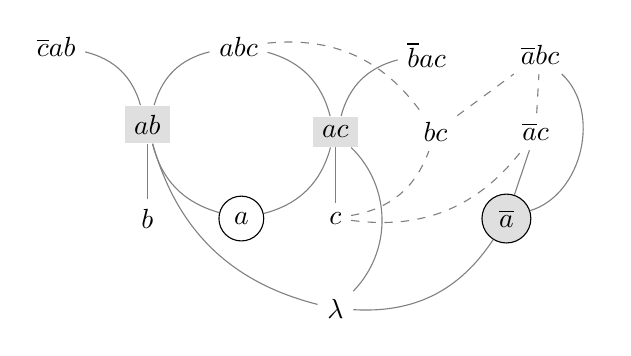
\begin{tikzpicture}[node distance=2em]
			\node[event] (E) {$\emptyevent$};
			\node[event, above = of E] (c) {$c$};
			\node[tchoice, left = of c] (a) {$a$};
			\node[event, left = of a] (b) {$b$};
			\node[right = of c] (invis) {};
			\node[smodel, above = of b] (ab) {$ab$};
			\node[smodel, above = of c] (ac) {$ac$};
			\node[event, above right = of ab] (abc) {$abc$};
			\node[event, above left = of ab] (abC) {$\co{c}ab$};
			\node[event, above right = of ac] (aBc) {$\co{b}ac$};
			\node[indep, right = of ac] (bc) {$bc$};
			\node[tchoice, smodel, right = of invis] (A) {$\co{a}$};
			\node[event, right = of bc] (Ac) {$\co{a}c$};
			\node[event, right = of aBc] (Abc) {$\co{a}bc$};
			% ----
			\draw[doubt] (a) to[bend left] (ab);
			\draw[doubt] (a) to[bend right] (ac);

			\draw[doubt] (ab) to[bend left] (abc);
			\draw[doubt] (ab) to[bend right] (abC);

			\draw[doubt] (ac) to[bend right] (abc);
			\draw[doubt] (ac) to[bend left] (aBc);

			\draw[doubt, dashed] (Ac) to (Abc);

			\draw[doubt] (A) to (Ac);
			\draw[doubt] (A) to[bend right=60] (Abc);

			\draw[doubt] (ab) to[bend right] (E);
			\draw[doubt] (ac) to[bend left=45] (E);
			\draw[doubt] (A) to[bend left] (E);

			\draw[doubt] (ab) to (b);
			\draw[doubt] (ac) to (c);
			\draw[doubt, dashed] (c) to[bend right] (bc);
			\draw[doubt, dashed] (abc) to[bend left] (bc);
			\draw[doubt, dashed] (bc) to (Abc);
			\draw[doubt, dashed] (c) to[bend right] (Ac);
		\end{tikzpicture}
	\end{center}

	\caption{%
		This (partial sub-/super-set) diagram shows some events related to
		the \aclp{SM} of the program \cref{eq:fruitful}.  The circle nodes
		are \aclp{TC} and shaded nodes are \aclp{SM}.  Solid lines
		represent relations with the \aclp{SM} and dashed lines some
		sub-/super-set relations with other events.  The set of events
		contained in all \aclp{SM}, denoted by $\consequenceclass$, is
		$\set{ \emptyevent }$ in this example, because
		$\co{a} \cap ab \cap ac = \emptyset = \emptyevent$.}
	\label{fig:ex:fruitful}
\end{figure}

The diagram in \cref{fig:ex:fruitful} illustrates the problem of propagating
probabilities from \aclp{TC} to \aclp{SM} and then to general events in an
\emph{edge-wise} process, \emph{i.e.}~where the value in a node is defined
from the values in its neighbors. This quickly leads to coherence problems
concerning probability, with no clear systematic approach. For example,
notice that $bc$ is not directly related with any \acl{SM}. Propagating
values through edges would assign a value ($\not= 0$) to $bc$ hard to explain
in terms of the semantics of the program. Instead, we propose to settle such
propagation on the relation an event has with the \aclp{SM}.

\subsection{An Equivalence Relation}
\label{subsec:equivalence.relation}
\begin{figure}[t]
	\begin{center}
		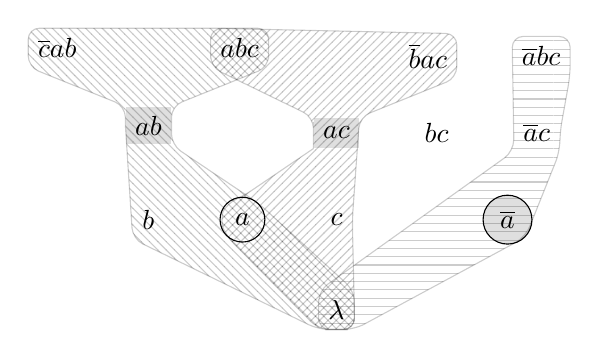
\begin{tikzpicture}[node distance=2em]
			\node[event] (E) {$\emptyevent$};
			\node[event, above = of E] (c) {$c$};
			\node[tchoice, left = of c] (a) {$a$};
			\node[event, left = of a] (b) {$b$};
			\node[right = of c] (invis) {};
			\node[smodel, above = of b] (ab) {$ab$};
			\node[smodel, above = of c] (ac) {$ac$};
			\node[event, above right = of ab] (abc) {$abc$};
			\node[event, above left = of ab] (abC) {$\co{c}ab$};
			\node[event, above right = of ac] (aBc) {$\co{b}ac$};
			\node[indep, right = of ac] (bc) {$bc$};
			\node[tchoice, smodel, right = of invis] (A) {$\co{a}$};
			\node[event, right = of bc] (Ac) {$\co{a}c$};
			\node[event, right = of aBc] (Abc) {$\co{a}bc$};
			% ----
			\path[draw, rounded corners, pattern=north west lines, opacity=0.2]
			(ab.west) -- (ab.north west) --
			(abC.south west) -- (abC.north west) -- (abC.north) --
			(abc.north east) -- (abc.east) -- (abc.south east) --
			(ab.north east) -- (ab.east) -- (ab.south east) --
			(a.north east) --
			(E.north east) -- (E.east) --
			(E.south east) -- (E.south) --
			(E.south west) --
			(b.south west) --
			(ab.west) ;
			% ----
			\path[draw, rounded corners, pattern=north east lines, opacity=0.2]
			(ac.south west) -- (ac.west) -- (ac.north west) --
			(abc.south west) -- (abc.west) -- (abc.north west) --
			(aBc.north east) -- (aBc.east) -- (aBc.south east) --
			(ac.north east) --
			(c.east) --
			(E.east) -- (E.south east) -- (E.south) -- (E.south west) --
			(a.south west) -- (a.west) -- (a.north west) -- (a.north) --
			(ac.south west) ;
			% ----
			\path[draw, rounded corners, pattern=horizontal lines, opacity=0.2]
			(Ac.west) --
			(Abc.north west) -- (Abc.north) --
			(Abc.north east) -- (Abc.south east) --
			(Ac.east) -- (Ac.south east) --
			(A.east) -- (A.south east) --
			(E.south east) -- (E.south) --
			(E.south west) -- (E.west) --
			(E.north west) --
			(Ac.south west) -- (Ac.west);
		\end{tikzpicture}
	\end{center}

	\caption{Classes of (consistent) events related to the \aclp{SM} of
		\cref{ex:fruitful} are defined through sub-/super-set relations.
		In this picture we can see, for example, that
		$\set{\co{c}ab, ab, b}$ and $\set{a, abc}$ are part of
		different classes, represented by different fillings.  As before,
		the circle nodes are \aclp{TC} and shaded nodes are \aclp{SM}. Notice that $bc$ is not in a filled area.}
	\label{fig:ex:fruitful.classes}
\end{figure}

\begin{figure}[t]
	\begin{center}
		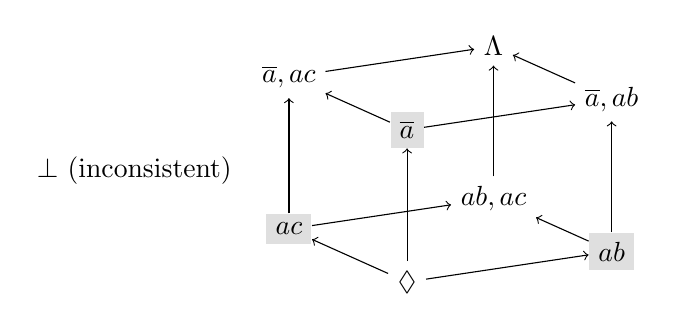
\begin{tikzpicture}[3d view]
			\node[event] (INDEPENDENT) at (0,0,0){$\indepclass$};
			\node[smodel] (A) at (0,0,2) {$\co{a}$};
			\node[smodel] (ab) at (3,0,0) {$ab$};
			\node[smodel] (ac) at (0,3,0) {$ac$};
			\node[event] (Aab) at (3,0,2) {$\co{a},ab$};
			\node[event] (Aac) at (0,3,2) {$\co{a},ac$};
			\node[event] (abac) at (3,3,0) {$ab,ac$};
			\node[event] (Aabac) at (3,3,2) {$\consequenceclass$};
			\node[event] (INCONSISTENT) at (-4, 0, 2) {$\inconsistent$
				(inconsistent)};
			% ----
			\draw[->] (INDEPENDENT) -- (A);
			\draw[->] (INDEPENDENT) -- (ab);
			\draw[->] (INDEPENDENT) -- (ac);
			\draw[->] (A) -- (Aab);
			\draw[->] (A) -- (Aac);
			\draw[->] (ab) -- (Aab);
			\draw[->] (ab) -- (abac);
			\draw[->] (ac) -- (Aac);
			\draw[->] (ac) -- (abac);
			\draw[->] (Aab) -- (Aabac);
			\draw[->] (Aac) -- (Aabac);
			\draw[->] (abac) -- (Aabac);
		\end{tikzpicture}
	\end{center}

	\caption{%
		Lattice of the \aclp{SC} from \cref{ex:fruitful}.  In this diagram
		the nodes are the different \aclp{SC} that result from the
		\aclp{SM}, plus the \emph{inconsistent} class ($\inconsistent$).
		The bottom node ($\indepclass$) is the class of
		\emph{independent} events, those that have no sub-/super-set
		relation with the \acp{SM} and the top node ($\consequenceclass$)
		represents events related with all the \acp{SM} \emph{i.e.}~the \emph{consequences} of the program.  As in previous
		diagrams, shaded nodes represent the \acp{SM}.}
	\label{fig:fruitful.lattice}
\end{figure}

Our path to propagate probabilities starts with the perspective that
\aclp{SM} play a role similar to \emph{prime factors} or \emph{principal
	ideals}. The \aclp{SM} of a program are the irreducible events entailed from
that program and any event must be considered under its relation with the
\aclp{SM}.

From \cref{ex:fruitful} and \cref{fig:ex:fruitful.classes} consider the
\aclp{SM} $\co{a}, ab, ac$ and events $a, abc$ and $c$. While $a$ is related
with (i.e.~contained in) both $ab, ac$, the event $c$ is related only with
$ac$. So, $a$ and $c$ are related with different \aclp{SM}. On the other
hand, $abc$ contains both $ab, ac$. So $a$ and $abc$ are related with the
same \aclp{SM}.

The \textit{\acf{SC}} of the event $e\in \EVENTSset$ is
\begin{equation}
	\stablecore{e} := \set{\, s \in \MODELset \given s \subseteq e \vee e \subseteq s\, } \label{eq:stable.core}
\end{equation}
where $\MODELset$ is the set of \aclp{SM}.

Observe that the minimality of \aclp{SM} implies that either $e$ is a
\acl{SM} or at least one of $\exists s \del{s \subseteq e}, \exists s \del{e
		\subseteq s}$ is false \emph{i.e.,}\ no \acl{SM} contains another.

\ifExamples
	\begin{example}[Stable cores]
		\label{ex:stable.cores}
		\em

		Continuing \cref{ex:fruitful}, depicted in
		\cref{fig:ex:fruitful,fig:ex:fruitful.classes,fig:fruitful.lattice}, and
		$\MODELset = \set{ab, ac, \co{a}}$, consider the following \aclp{SC} of some
		events:
		\begin{equation*}
			\begin{aligned}
				\stablecore{a}           & = \set{s \in \MODELset \given s \subseteq a \vee a \subseteq s}                                        & = \set{ab, ac}      %
				\\
				\stablecore{abc}         & = \set{s \in \MODELset \given s \subseteq abc \vee abc \subseteq s}                                    & = \set{ab, ac}      %
				\\
				\stablecore{\co{c}ab}    & = \set{s \in \MODELset \given s \subseteq \co{c}ab \vee \co{c}ab \subseteq s}                          & = \set{ab}          %
				\\
				\stablecore{bc}          & = \set{s \in \MODELset \given s \subseteq bc \vee bc \subseteq s}                                      & = \emptyset         %
				\\
				\stablecore{\emptyevent} & = \set{s \in \MODELset \given s \subseteq \emptyset \vee \emptyset \subseteq s} = \set{ab, ac, \co{a}} & = \consequenceclass %
				\\
			\end{aligned}
		\end{equation*}

		Events $a$ and $abc$ have the same \ac{SC}, while $\co{c}ab$ has a different
		\ac{SC}. Also, $bc$ is \emph{independent of} (\emph{i.e.}\ not related to)
		any \acl{SM}. Since events are sets of literals, the empty set is an event
		and a subset of any \ac{SM}.
	\end{example}
\fi

We now define an equivalence relation so that two events are related if
either both are inconsistent or both are consistent and, in the latter case,
with the same \acl{SC}.
\begin{definition}[Equivalence Relation on Events.]\label{def:equiv.rel}

	For a given program, let $u, v \in \EVENTSset$. The equivalence relation
	$\sim$ is defined by
	\begin{equation}
		u \sim v\ :\clause\ u,v \not\in\CONSISTset \vee \del{u,v \in \CONSISTset \wedge \stablecore{u} = \stablecore{v}}.\label{eq:equiv.rel}
	\end{equation}

\end{definition}

This equivalence relation defines a partition on the set of events, where
each class holds a unique relation with the \aclp{SM}. In particular we
denote each class by:
\begin{equation}
	\class{e} =
	\begin{cases}
		\inconsistent := \EVENTSset \setminus \CONSISTset
		 & \text{if~} e \in \EVENTSset \setminus \CONSISTset, %
		\\
		\set{u \in \CONSISTset \given \stablecore{u} = \stablecore{e}}
		 & \text{if~} e \in \CONSISTset.
	\end{cases}\label{eq:event.class}
\end{equation}

\begin{proposition}[Class of the Program's Consequences]
	\label{prop:consequence.class}
	Let $\emptyevent$ be the event empty set (because
	$\emptyset \in \EVENTSset$), and $\consequenceclass$ the
	\emph{consequence class} of events related with all the
	\aclp{SM}.  Then
	\begin{equation}
		\class{\emptyevent} = \stablecore{\MODELset} = \consequenceclass.
	\end{equation}
\end{proposition}

The combinations of \aclp{SM}, \textit{i.e.}~the \aclp{SC}, together with the
set of inconsistent events ($\inconsistent$) forms a set of representatives
for the equivalence relation $\sim$. Since all events within an equivalence
class have the same relation with a specific \acl{SC}, we are interested in
functions (including probability distributions), that are constant within
classes. A function $f:\EVENTSset\to Y$, where $Y$ is any set, is said to be
\emph{coherent} if
\begin{equation}
	\forall u\in \class{e} \left( f\at{u} = f\at{e} \right).
\end{equation}

Considering coherent functions, in the specific case of \cref{eq:fruitful},
instead of dealing with the $2^6 = 64$ events, we need to consider only the
$2^3 + 1 = 9$ classes, well defined in terms of combinations of the
\aclp{SM}, to define coherent functions. In general, a program with $n$ atoms
and $m$ \aclp{SM} has $2^{2n}$ events and $2^m + 1$ \aclp{SC}.

\ifExamples
	\begin{example}[Events classes]\label{ex:classes}\em

		Consider again \cref{ex:fruitful}. As previously stated, the \aclp{SM} are
		the elements of $\MODELset = \set{\co{a}, ab, ac}$ so the quotient set of
		this relation is
		\begin{equation*}
			\class{\EVENTSset} = \set{
				\begin{array}{lll}
					\inconsistent,           &
					\indepclass,             &
					\stablecore{\co{a}},%
					\\
					\stablecore{ab},         &
					\stablecore{ac},         &
					\stablecore{\co{a}, ab},%
					\\
					\stablecore{\co{a}, ac}, &
					\stablecore{ab, ac},     &
					\consequenceclass
				\end{array}
			},
		\end{equation*}
		where $\indepclass$ denotes the class of \emph{independent
			events} $e$ such that $\stablecore{e} = \set{\emptyset}$,
		while $\consequenceclass = \stablecore{\MODELset}$ is the set of
		events related with all \acp{SM}.  We have:
		\begin{equation*}
			\begin{array}{l|lr}
				\stablecore{e}
				       & \class{e}
				       & \# \class{e}                                                                           %
				\\
				\hline
				%
				\inconsistent
				       & \co{a}a, \ldots
				       & 37                                                                                     %
				\\
				%
				\indepclass
				       & \co{b}, \co{c}, bc, \co{b}a, \co{b}c, \co{bc}, \co{c}a, \co{c}b, \co{bc}a
				       & 9                                                                                      %
				\\
				%
				\co{a}
				       & \co{a}, \co{a}b, \co{a}c, \co{ab}, \co{ac}, \co{a}bc, \co{ac}b, \co{ab}c, \co{abc}
				       & 9                                                                                      %
				\\
				%
				ab     & b, ab, \co{c}ab                                                                    & 3 \\%%
				%
				ac     & c, ac, \co{b}ac                                                                    & 3 \\%%
				%
				\co{a}, ab
				       &
				       & 0                                                                                      %
				\\
				%
				\co{a}, ac
				       &
				       & 0
				%
				\\
				%
				ab, ac & a, abc                                                                             & 2 \\%%
				%
				\consequenceclass
				       & \emptyevent
				       & 1
				\\
				%
				\hline \class{\EVENTSset}
				       & \EVENTSset
				       & 64
			\end{array}
		\end{equation*}

		Notice that $bc \in \indepclass$, as hinted by
		\cref{fig:ex:fruitful,fig:ex:fruitful.classes}.
	\end{example}
\fi

\subsection{From Total Choices to Events}
\label{subsec:from.tchoices.to.events}

Our path to set a distribution on $\EVENTSset$ continues with the more
general problem of extending \emph{measures}, since propagating
\emph{probabilities} easily follows by means of a suitable normalization
(done in \cref{eq:measure.events.unconditional,eq:probability.event}), and
has two phases: (1) Propagation of the probabilities, \emph{as measures},
from the \aclp{TC} to events and (2) Normalization of the measures on events,
recovering a probability.

The ``propagation'' phase, traced by \cref{eq:prob.total.choice} and
\crefrange{eq:measure.tchoice}{eq:measure.events.unconditional}, starts with
the probability (as a measure) of \aclp{TC}, $\pwt{t} = \prT\at{t}$,
propagates it to the \aclp{SM}, $\pwm{s}$, and then, within the equivalence
relation from \cref{eq:equiv.rel}, to a coherent measure of events,
$\pwe{e}$, including (consistent) worlds. So we are specifying a sequence of
functions
\begin{equation}
	\pwT , \pwM , \pwC , \pwE\label{eq:sequence.functions}
\end{equation}
on successive larger domains
\(
\TCHOICEset , \MODELset , \class{\EVENTSset} , \EVENTSset
\)
so that the last function ($\pwE$) is a finite coherent measure on
the set of events and thus, as a final step, it can easily be used to
define a probability distribution of events by normalization:
\(
\pwE \longrightarrow \prE
\).

\subsubsection*{Total Choices and Stable models}
\label{par:prop.totalchoices}

Let's start by looking into the first two steps of the sequence of functions
\cref{eq:sequence.functions}: $\pwT$ and $\pwM$. Using
\cref{eq:prob.total.choice}, the measure $\mu_{\cal T}$ of the \acl{TC} $t
	\in \TCHOICEset$ is given by
\begin{equation}
	\pwt{t} := \prT\at{t}=
	\prod_{\substack{
			\probfact{a}{p}~ \in ~\PROBFset,%
	\\
			a~ \in~ t}} p\ \ \times\
	\prod_{\substack{
			\probfact{a}{p}~ \in ~\PROBFset,%
	\\
			\co{a}~\in~ t}} \co{p}.
	\label{eq:measure.tchoice}
\end{equation}

Recall that each \acl{TC} $t \in \TCHOICEset$, together with the rules and
the other facts of a program, defines the set \tcgen{t} of \aclp{SM}
associated with that choice. Given a \acl{TC} $t \in \TCHOICEset$, a \acl{SM}
$s \in \MODELset $, and formal variables or values $\theta_{s,t} \in
	\intcc{0, 1}$ such that $\sum_{s\in \tcgen{t}} \theta_{s,t} = 1$, we define
\begin{equation}
	\pwm{s, t} := \begin{cases}
		              \theta_{s,t} & \text{if~} s \in \tcgen{t}\cr 0 & \text{otherwise.}
	              \end{cases}
	\label{eq:measure.stablemodel}
\end{equation}

The $\theta_{s,t}$ parameters in \cref{eq:measure.stablemodel} express the
\emph{program's} lack of information about the measure assignment, when a
single \acl{TC} entails more than one \acl{SM}. We propose to address this
issue by assigning a possibly unknown parameter, \textit{i.e.}~a formal
variable, ($\theta_{s,t}$) associated with a \acl{TC} ($t$) and a \acl{SM}
($s$). This allows the expression of a quantity that does not result from the
program but might be determined or estimated given more information,
\textit{e.g.} observed data.

As sets, the \aclp{SM} can have non-empty intersection. But because different
\acp{SM} represent different states of a system, we assume that the algebra
of the \aclp{SM} is $\sigma$-additive:

\begin{assumption}[\Aclp{SM} as Disjoint Observations.]
	\label{assumption:smodels.disjoint}%

	For any set $X$ of \aclp{SM} and any \acl{TC} $t$,
	\begin{equation}
		\pwM\at{X, t} = \sum_{s\in X}\pwM\at{s, t}.\label{eq:smodels.disjoint}
	\end{equation}

\end{assumption}

\Cref{eq:smodels.disjoint} is the basis for \cref{eq:measure.class.consistent} and effectively extends $\pwM:\MODELset \to \mathbb{R}$ to $\pwM:\powerset{\MODELset} \to \mathbb{R}$. Notice that the pre-condition of \cref{eq:measure.stablemodel} can now be stated as $\pwM\at{\MODELset\at{t}, t} = 1$.

\ifExamples
	\begin{example}[\Aclp{SM} and parameters]
		\label{ex:models.parameters}
		\em

		The program from \cref{ex:fruitful} has no information about the
		probabilities of the \aclp{SM} that result from the \acl{TC} $t = \set{a}$.
		These models are $\MODELset\at{\set{a}} = \set{ab, ac}$ so we need two
		parameters $\theta_{ab, \set{a}}, \theta_{ac, \set{a}} \in \intcc{0,1}$ and
		such that (\textit{cf.}\ \cref{eq:measure.stablemodel})
		\begin{equation*}
			\theta_{ab, \set{a}} + \theta_{ac, \set{a}} = 1.
		\end{equation*}

		If we let $\theta = \theta_{ab, \set{a}}$ then
		\begin{equation*}
			\theta_{ac, \set{a}} = 1 - \theta = \co{\theta}.
		\end{equation*}

		Also
		\begin{equation*}
			\begin{split}
				\theta_{ab, \set{\co{a}}} & = 0, %
				\\
				\theta_{ac, \set{\co{a}}} & = 0
			\end{split}
		\end{equation*}
		because $ab, ac \not\in\MODELset\at{\co{a}}$.
	\end{example}
\fi

\subsubsection*{Classes}
\label{par:prop.class.cases}

Consider the next function in sequence \cref{eq:sequence.functions}, $\pwC$
on $\class{\EVENTSset}$. Each class of the equivalence relation $\sim$
(eq.~\ref{eq:equiv.rel}) is either the inconsistent class ($\inconsistent$)
or is associated with a \acl{SC}, \textit{i.e.~}a set of \aclp{SM}.
Therefore, $\pwC$ is defined considering the following two cases:
\paragraph{Inconsistent class.} This class contains events that are logically
inconsistent, thus should never be observed and thus have measure zero:
\begin{equation}
	\pwc{\inconsistent, t} := 0.
	\footnote{This measure being zero is independent of the \acl{TC}.}
	\label{eq:measure.class.inconsistent}
\end{equation}
\paragraph{Consistent classes.} For the propagation function to be coherent, it
must be constant within a class and its value dependent only on the \acl{SC}:
\begin{subequations}
	\begin{equation}
		\pwc{\class{e}, t} := \pwm{\stablecore{e}, t} = \sum_{s\in\stablecore{e}}\pwm{s, t}.
		\label{eq:measure.class.consistent}
	\end{equation}
	and we further define the following:
	\begin{equation}
		\pwc{\class{e}} := \sum_{t \in \TCHOICEset} \pwt{t}\pwc{\class{e}, t}
		\label{eq:measure.class.unconditional}
	\end{equation}
\end{subequations}
\Cref{eq:measure.class.consistent} states that the measure of a
class $\class{e}$ is the measure of its \acl{SC}
($\stablecore{e}$) and \cref{eq:measure.class.unconditional}
\emph{averages} \cref{eq:measure.class.consistent} over the
\aclp{TC}.

Notice that \cref{eq:measure.class.consistent} also applies to the
independent class, $\indepclass$, because events in this class are not
related with any \acl{SM}. For such an event $e$, $\stablecore{e} =
	\emptyset$ so
\begin{equation}
	\pwc{\indepclass, t} = \sum_{s\in\emptyset}\pwm{s, t} = 0.
	\label{eq:measure.class.independent}
\end{equation}

\ifExamples
	\begin{example}[Measure of \aclp{SM} and classes]\label{ex:measures.sm}\em
		\begin{equation*}
			\begin{array}{c||l|ccc|ccc|c|c|r}
				%=====================================================
				  &
				A & B                                         & C      & D           & E & F & G & H & I & J
				\\[3pt]
				\hline
				\hline
				\multirow{3}{*}{\phantom{2em}}
				  & \multirow{3}{*}{\stablecore{e}}
				  & \multicolumn{3}{c|}{\pwm{s,\set{\co{a}}}}
				  & \multicolumn{3}{c|}{\pwm{s,\set{a}}}
				  & \pwc{\class{e},\set{\co{a}}}
				  & \pwc{\class{e},\set{a}}
				  & \multirow{3}{*}{\pwc{\class{e}}}
				\\[2pt]
				%=====================================================
				  &
				  & \co{a}                                    & ab     & ac
				  & \co{a}                                    & ab     & ac
				  & \pwt{\set{\co{a}}}
				  & \pwt{\set{a}}
				  &
				\\[2pt]
				%=====================================================
				  &
				  & 1                                         & 0      & 0
				  & 0                                         & \theta & \co{\theta}
				  & 0.7
				  & 0.3
				  &
				\\[3pt]
				%=====================================================
				\hline
				1
				  & \co{a}
				  & 1                                         &        &
				  & 0                                         &        &
				  & 1
				  & 0
				  & 0.7
				\\[2pt]
				%=====================================================
				2
				  & ab
				  &                                           & 0      &
				  &                                           & \theta &
				  & 0
				  & \theta
				  & 0.3\theta
				\\[2pt]
				%=====================================================
				3
				  & ac
				  &                                           &        & 0
				  &                                           &        & \co{\theta}
				  & 0
				  & \co{\theta}
				  & 0.3\co{\theta}
				\\[2pt]
				%=====================================================
				4
				  & \co{a}, ab
				  & 1                                         & 0      &
				  & 0                                         & \theta &
				  & 1
				  & \theta
				  & 0.7 + 0.3\theta
				\\[2pt]
				%=====================================================
				5
				  & \co{a}, ac
				  & 1                                         &        & 0
				  & 0                                         &        & \co{\theta}
				  & 1
				  & \co{\theta}
				  & 0.7 + 0.3\co{\theta}
				\\[2pt]
				%=====================================================
				6
				  & ab, ac
				  &                                           & 0      & 0
				  &                                           & \theta & \co{\theta}
				  & 0
				  & \theta + \co{\theta} = 1
				  & 0.3
				\\[2pt]
				%=====================================================
				7
				  & \consequenceclass
				  & 1                                         & 0      & 0
				  & 0                                         & \theta & \co{\theta}
				  & 1
				  & \theta + \co{\theta} = 1
				  & 1
				%=====================================================
			\end{array}
		\end{equation*}

		Continuing \cref{ex:fruitful}, we show the propagation of $\pwT$ to $\pwM$
		(\cref{eq:measure.tchoice}) and then to $\pwC$
		(\cref{eq:measure.class.consistent,eq:measure.class.unconditional}). The
		table above resumes the calculations to compute $\pwc{\class{e}}$ for each $e
			\in \EVENTSset$. For example, $e = abc$ the calculation of $J6 =
			\pwc{\class{abc}}$ follows these steps:
		\begin{enumerate}
			\item $\stablecore{abc} = \set{ab,ac}$ --- is in line $6$ of the table.
			\item Since $\TCHOICEset = \set{\set{a}, \set{\co{a}}}$, we need to calculate $I6 =
				      \pwc{\class{abc}, \set{a}}$ and $H6 = \pwc{\class{abc}, \set{\co{a}}}$. By
			      \cref{eq:measure.class.consistent}:
			      \begin{equation*}
				      \begin{aligned}
					      H6 = \pwc{\class{abc}, \set{\co{a}}}
					       & = \sum_{s \in \stablecore{abc}} \pwm{s, \set{\co{a}}}
					      =
					       & \pwm{ab, \set{\co{a}}} +  \pwm{ac, \set{\co{a}}}      %
					      \\
					      I6 = \pwc{\class{abc}, \set{a}}
					       & = \sum_{s \in \stablecore{abc}} \pwm{s, \set{a}}
					      =
					       & \pwm{ab, \set{a}} +  \pwm{ac, \set{a}}
				      \end{aligned}
			      \end{equation*}
			\item The $\pwm{s,t}$ above result from \cref{eq:measure.stablemodel} --- the
			      non-empty cells in columns $B:D$ and $E:G$:
			      \begin{equation*}
				      \begin{aligned}
					      C6
					       & = \pwm{ab, \set{\co{a}}}
					       & = 0                      %
					      \\
					      D6
					       & = \pwm{ac, \set{\co{a}}}
					       & = 0                      %
					      \\
					      F6
					       & = \pwm{ab, \set{a}}
					       & = \theta                 %
					      \\
					      G6
					       & = \pwm{ac, \set{a}}
					       & = \co{\theta}
				      \end{aligned}
			      \end{equation*}
			\item So we have --- columns $H, I$:
			      \begin{equation*}
				      \begin{aligned}
					      H6
					       & = \pwc{\class{abc}, \set{\co{a}}}
					       & = 0 + 0
					       &
					       & = 0                               %
					      \\
					      I6
					       & = \pwc{\class{abc}, \set{a}}
					       & = \theta + \co{\theta}
					       &
					       & = 1
				      \end{aligned}
			      \end{equation*}
			\item At last, by \cref{eq:measure.class.unconditional} --- columns $H, I$ and $J$:
			      \begin{equation*}
				      \begin{split}
					      J6 = \pwc{\class{abc}}
					       & = \sum_{t\in\MODELset} \pwc{\class{abc}, t}\pwt{t}                %
					      \\
					       & =  \pwc{\class{abc}, \set{\co{a}}}\pwt{\set{\co{a}}} +
					      \pwc{\class{abc}, \set{a}}\pwt{\set{a}}%
					      \\
					       & =  0 \co{\theta} +  1 \theta =  0 \times 0.7 +  1\times 0.3 = 0.3
				      \end{split}
			      \end{equation*}
		\end{enumerate}
	\end{example}
\fi

\subsubsection*{Events and Probability}
\label{par:propagation.event.cases}

Each consistent event $e \in \EVENTSset$ is in the class defined by its
\acl{SC} $\stablecore{e}$. So, denoting the number of elements in $X$ as $\#
	X$, we set:
\begin{subequations}
	\begin{equation}
		\pwe{e, t} :=
		\begin{cases}
			\frac{\pwc{\class{e}, t}}{\# \class{e}} & \text{if~}\# \class{e} > 0, %
			\\
			0                                       & \text{otherwise}.
		\end{cases}
		\label{eq:measure.events}
	\end{equation}
	and, by averaging over the \aclp{TC}:
	\begin{equation}
		\pwe{e} := \sum_{t\in\TCHOICEset} \pwt{t}\pwe{e, t}.
		\label{eq:measure.events.unconditional}
	\end{equation}
\end{subequations}
In order to get a probability from \cref{eq:measure.events.unconditional}, we need a \emph{normalizing factor}:
\begin{equation}
	Z :=
	\sum_{e \in \EVENTSset} \pwe{e} =
	\sum_{\class{e} \in \class{\EVENTSset}} \pwc{\class{e}},\label{eq:normalizing.factor}
\end{equation}
and now \cref{eq:measure.events.unconditional} provides a
straightforward way to define the \emph{probability of a
	single event $e \in \EVENTSset$}:
\begin{equation}
	\prE\at{e} := \frac{\pwe{e}}{Z}.\label{eq:probability.event}
\end{equation}

\Cref{eq:probability.event} defines a coherent \emph{prior}\footnote{In the Bayesian sense that future observations might update this probability.}
probability of events and, together with external statistical
knowledge, can be used to learn about the \emph{initial} probabilities
of the literals, that should not (and by \cref{prop:two.distributions}
can't) be confused with the explicit $\pwT$ set in the program.

\ifExamples
	\begin{example}[Coherent probability of events]\label{ex:choerent.probability}\em

		In \cref{ex:measures.sm} we determined $\pwc{\class{e}, t}$ from
		\cref{eq:measure.class.consistent} and also $\pwc{\class{e}}$, the measure of
		each class, using \cref{eq:measure.class.unconditional}, that marginalizes
		the \aclp{TC}.
		\begin{equation*}
			\begin{array}{l|cc|c|c}
				\stablecore{e}
				       & \hspace{1em}\pwC\hspace{1em}
				       & \hspace{1em}\#\class{e}\hspace{1em}
				       & \hspace{1em}\pwE\hspace{1em}
				       & \hspace{1em}\prE\hspace{1em}
				\\
				\hline
				%
				\inconsistent
				       & 0
				       & 37
				       & 0
				       & 0
				\\[4pt]
				%
				\indepclass
				       & 0
				       & 9
				       & 0
				       & 0
				\\[4pt]
				%
				\co{a}
				       & \frac{7}{10}
				       & 9
				       & \frac{7}{90}
				       & \frac{7}{207}
				\\[4pt]
				%
				ab     & \frac{3}{10}\theta                  & 3 & \frac{1}{10}\theta      & \frac{1}{23}\theta \\[4pt]
				%
				ac     & \frac{3}{10}\co{\theta}             & 3 & \frac{1}{10}\co{\theta} &
				\frac{1}{23}\co{\theta}                                                                         \\[4pt]
				%
				\co{a}, ab
				       & \frac{7 + 3\theta}{10}
				       & 0
				       & 0
				       & 0
				\\[4pt]
				%
				\co{a}, ac
				       & \frac{7 + 3\co{\theta}}{10}
				       & 0
				       & 0
				       & 0
				\\[4pt]
				%
				ab, ac & \frac{3}{10}                        & 2 & \frac{3}{20}            & \frac{3}{46}       \\[4pt]
				%
				\consequenceclass
				       & 1
				       & 1
				       & 1
				       & \frac{10}{23}
				\\[4pt]
				%
				\hline
				       &
				       &
				       &
				       &
				\\[-0.5em]
				       & Z = \frac{23}{10}
				       &
				       & \frac{\pwC}{\#\class{e}}
				       & \frac{\pwE}{X}
				%& \Sigma = 1 
			\end{array}
		\end{equation*}

		From there we can follow \cref{eq:measure.events} to calculate the measure
		$\pwe{e, t}$ of each event given $t$, by simply dividing $\pwc{\class{e}, t}$
		by $\#\class{e}$, the total number of elements in $\class{e}$. Then we
		marginalize $t$ in $\pwe{e, t}$ to get $\pwe{e}$. Finally, the normalization
		factor from \cref{eq:normalizing.factor} and \cref{eq:probability.event}
		provide a coherent \emph{prior} probability for each event.

		In summary, the coherent \emph{prior} probability of events of program
		\cref{eq:fruitful} is
		\begin{equation}
			\begin{array}{l|ccccccccc}
				\stablecore{e}          &
				\inconsistent           &
				\indepclass             &
				\co{a}                  &
				ab                      &
				ac                      &
				\co{a}, ab              &
				\co{a}, ac              &
				ab, ac                  &
				\consequenceclass
				\\ \hline
				\prE\at{e}              &
				0                       &
				0                       &
				\frac{7}{207}           &
				\frac{1}{23}\theta      &
				\frac{1}{23}\co{\theta} &
				0                       &
				0                       &
				\frac{3}{46}            &
				\frac{10}{23}
			\end{array}
		\end{equation}
		\label{eq:sbf.prior}

	\end{example}
\fi

Now $\prE:\EVENTSset \to \intcc{0,1}$ can be extended to
$\prE:\powerset{\EVENTSset}\to\intcc{0,1}$ by abusing notation and setting,
for $X \subseteq \EVENTSset$,
\begin{equation}
	\prE\at{X} = \sum_{x\in X}\prE\at{x}.
	\label{eq:prob.event.set}
\end{equation}
It is straightforward to verify that the latter satisfies the Kolmogorov
axioms of probability.

We can now properly state the following property about \emph{certain facts}
such as $\probfact{a}{1.0}$.
\begin{proposition}[Probability of Certain Facts.]
	\label{prop:prob.one}

	Consider a program $A$ with the probabilistic fact $\probfact{a}{1.0}$ and
	$A'$ where it is replaced by the deterministic fact $a$. Let $\prE$ be as
	\cref{eq:probability.event} for $A$ and $\prfunc'_{\EVENTSset}$ for $A'$.
	Then
	\begin{equation}
		\forall e \in \EVENTSset \left(\prE\at{e} = \prfunc'_{\EVENTSset}\at{e}\right).
	\end{equation}
\end{proposition}

Since \aclp{TC} are also events, one can ask, for an arbitrary \acl{TC} $t$,
if $\prT\at{t} = \prE\at{t}$ or, equivalently, if $\pwt{t} = \pwe{t}$.
However, it is easy to see that, in general, this cannot be true. While the
domain of $\prT$ is the set of \aclp{TC}, for $\prE$ the domain is much
larger, including all the events. Except for trivial programs, where the
\acp{SM} are the \acp{TC}, some events other than \aclp{TC} will have
non-zero probability.
\begin{proposition} \label{prop:two.distributions} %

	If a program has a \acl{SM} that is not a \acl{TC} then there is at least one
	$t\in\TCHOICEset$ such that
	\begin{equation}
		\prT\at{t} \not= \prE\at{t}. \label{eq:two.distributions}
	\end{equation}

\end{proposition}
\begin{proof}
	Suppose towards a contradiction that $\prT\at{t} = \prE\at{t}$ for
	all $t \in \TCHOICEset$.  Then
	\begin{equation*}
		\sum_{t\in\TCHOICEset} \prE\at{t} = \sum_{t\in\TCHOICEset} \prT\at{t} = 1.
	\end{equation*}

	Hence $\prE\at{x} = 0$ for all $x \in \EVENTSset\setminus\TCHOICEset$, in
	contradiction with the fact that at least for one $s \in
		\MODELset\setminus\TCHOICEset$ it must be $\prE\at{s} > 0$.
\end{proof}

The essential, \emph{counter-intuitive}, conclusion of
\cref{prop:two.distributions} is that we are dealing with \emph{two
	distributions}: one, restricted to the \aclp{TC}, is explicit in the
annotations of the programs while the other, covering all the events, results
from the explicit annotations of the program \emph{and the structure of the
	\aclp{SM}}. For example:
\begin{equation*}
	\begin{aligned}
		\prT\at{a} & = 0.3          &  &
		\text{from the program \cref{ex:fruitful}}, %
		\\
		\prE\at{a} & = \frac{3}{64} &  &
		\text{from \cref{eq:sbf.prior}}.
	\end{aligned}
\end{equation*}
\begin{example}[Probability of Events]
	\label{ex:prob.events}
	\em
	In summary, for \cref{ex:fruitful}, the coherent \emph{prior} probability of
	events of program \cref{eq:fruitful} is
	\begin{equation}
		\begin{array}{l|ccccccccc}
			\stablecore{e}          &
			\inconsistent           &
			\indepclass             &
			\co{a}                  &
			ab                      &
			ac                      &
			\co{a}, ab              &
			\co{a}, ac              &
			ab, ac                  &
			\consequenceclass
			\\ \hline
			\prE\at{e}              &
			0                       &
			0                       &
			\frac{7}{207}           &
			\frac{1}{23}\theta      &
			\frac{1}{23}\co{\theta} &
			0                       &
			0                       &
			\frac{3}{46}            &
			\frac{10}{23}
		\end{array}
		\label{eq:sbf.prior}
	\end{equation}

	We can use this table to compute the probability of any single event $e \in
		\EVENTSset$ by looking at the column of the event's \acl{SC}. For example:
	\begin{description}
		\item $\prE\at{ab} = \frac{\theta}{23}, $ because $ab$ is the only \ac{SM} related with $ab$ so $\stablecore{ab} = \set{ab}$ and the probability value is found in the respective column of \cref{eq:sbf.prior}.

		\item $\prE\at{abc} = \frac{3}{46}$ because $abc \supset  ab$ and $abc \supset ac$. So $\stablecore{abc} = \set{ab, ac}$.

		\item $\prE\at{bc} = 0$ because, since there is no \ac{SM} $s$ that either $s \subset bc$ or $bc \subset s$, $\stablecore{bc} = \emptyset$ \emph{i.e.}\ $bc \in \indepclass$.

		\item $\prE\at{\co{a}b} = \frac{7}{207}$ because $\stablecore{\co{a}b} = \set{\co{a}}$.

		\item $\prE\at{\co{a}} = \frac{7}{207}$ and  $\prE\at{a} = \frac{3}{46}$. Notice that
		      $ \prE\at{\co{a}} + \prE\at{a} \not= 1. $
		      This highlights the fundamental difference between $\prE$ and $\prT$ (\emph{cf.~}\cref{prop:two.distributions}), where the former results from the lattice of the \aclp{SC} and the latter directly from the explicit assignment of probabilities to literals.
	\end{description}

	Related with the last case above, consider the complement of a consistent
	event $e$, denoted by $\complement e$. To calculate $\prE\at{\complement e}$
	we look for the classes in $\class{\EVENTSset}$ that are not $\class{e}$, \textit{i.e.}~the complement of $e$'s class within
	$\class{\EVENTSset}$\footnote{All the usual set operations hold on the
		complement. For example, $\complement\complement X = X$.},
	$\complement\class{e}$. Considering that $\class{\EVENTSset}$ is in a
	one-to-one correspondence with the \aclp{SC} plus $\inconsistent$, 
	\begin{equation*}
		\class{\EVENTSset} \simeq \set{
			\inconsistent, \indepclass, \set{\co{a}}
			, \set{ab}, \set{ac}, \set{\co{a}, ab}
			, \set{\co{a}, ac}, \set{ab, ac}, \consequenceclass}.
	\end{equation*}
	In particular for $\prE\at{\complement a}$, since $\stablecore{a} = \set{ab, ac}$ then $\complement \class{a} = \class{\EVENTSset} \setminus \class{a}$ and
	\(
	\prE\at{\complement a} =  \prE\at{\class{\EVENTSset} \setminus \class{a}} = 1 - \prE\at{a}
	\).
	Also, $\prE\at{\complement \co{a}} =  1 - \prE\at{\co{a}} $.
\end{example}

While not illustrated in our examples, this method also applies to programs
that have more than one \acl{PF}, like
\begin{equation*}
	\begin{aligned}
		\probfact{a & }{0.3},             %
		\\
		\probfact{b & }{0.6},             %
		\\
		c \vee d    & \clause a \wedge b.
	\end{aligned}
\end{equation*}

Our approach generalizes to Bayesian networks in a way similar to
\cite{cozman2020joy,raedt2016statistical} and
\cite{kiessling1992database,thone1997increased} as follows. On the one hand,
any acyclic propositional program can be viewed as the specification of a
Bayesian network over binary random variables. So, we may take the structure
of the Bayesian network to be the dependency graph. The random variables then
correspond to the atoms and the probabilities can be read off of the
probabilistic facts and rules. Conversely, any Bayesian network over binary
variables can be specified by an acyclic non-disjunctive \ac{SASP}.

\section{Discussion and Future Work}
\label{sec:discussion}

This work is a first venture into expressing probability distributions using
algebraic expressions derived from a logical program, in particular an
\ac{ASP}. We would like to point out that there is still much to explore
concerning the full expressive power of logic programs and \ac{ASP} programs.
So far, we have not considered recursion, logical variables or functional
symbols. Also, there is still little effort to articulate with the related
fields of probabilistic logical programming, machine learning, inductive
programming, \emph{etc.}

The equivalence relation from \cref{def:equiv.rel} identifies the $s
	\subseteq e$ and $e \subseteq s$ cases. Relations that distinguish such cases
might enable better relations between the models and processes from the
\aclp{SM}.

The theory, methodology, and tools, from Bayesian Networks can be adapted to
our approach. The connection with Markov Fields \cite{kindermann80} is left
for future work. An example of a ``program selection'' application (as
mentioned in \cref{item:program.selection},
\cref{ssec:propagating.probabilities}) is also left for future work.

We decided to set the measure of inconsistent events to $0$ but, maybe, in
some cases, we shouldn't. For example, since observations may be affected by
noise, one can expect inconsistencies between the literals of an observation
to occur.

\section*{Acknowledgements}

This work is partly supported by Funda\c{c}\~ao para a Ci\^{e}ncia e
Tecnologia (FCT/IP) under contracts UIDB/04516/2020 (NOVA LINCS),
UIDP/04674/2020 and UIDB/04675/2020 (CIMA).

The authors are grateful to Lígia Henriques-Rodrigues, Matthias Knorr and
Ricardo Gonçalves for valuable comments on a preliminary version of this
paper, and Alice Martins for contributions on software development.

\ifLNCS \bibliographystyle{splncs04} \fi
\ifTLP%
	\ifTLPBIB
		\bibliographystyle{tlplike}
	\else
		\bibpunct{(}{)}{;}{a}{}{;}
		\bibliographystyle{kluwer}
	\fi
\fi

\bibliography{zugzwang}
\end{document}

